\chapter{Iteración 3: Primer prototipo de Hardware} % (fold)
\label{cha:iteracion_3}


\section{Introducción} % (fold)
\label{it3:sec:introduccion}

Para realizar las pruebas en la iteracion anterior, utilizamos una placa de desarrollo Silicon Labs (modelo C8051f352DK). Esta placa de desarrollo es suficiente para albergar nuestro programa y funcionar como la plataforma de instrumentacion que intentamos construir. Pero, su tamaño y su precio no justifican su uso. En esta iteracion, nos enfocaremos en diseñar un circuito optimizado en base al mismo circuito que tiene esta placa de desarrollo; teniendo en cuenta aquellas funcionalidades que utilizamos para nuestra plataforma, y descartando aquellas que no sean necesarias. De esta manera, obtendremos un PCB optimizado, mas pequeño, y de menor costo.


%la primera placa que fue una verga. tenia el rs232, tenia 8 entradas, tenia la alimentacion separada de la entrada para la programacion del micro. osea podia alimentarse mediante el debugger o alimentacion externa. se adapto el diseño de la placa para poder programar el micro con el debugger de silicon labs. hay que tener en cuenta que nos basamos en el diseño hecho por silicon labs de la placa de desarrollo c8051f352 que teniamos en el lac. la vamos a haber construido en esta iteracion, y lo unico que llego a hacer fue conectarse con la ide. nada mas, el resto no anduvo nada. %

% section introduccion (end)

\section{Requerimientos de la iteracion} % (fold)
\label{it3:sec:requerimientos_de_la_iteracion}

Diseñar y construir un prototipo de placa que cumpla con los siguientes requerimientos:

\begin{itemize}
\item Al circuito se le deberian poder conectar 8 entradas analógicas.
\item Al circuito se le deberian poder conectar 4 entradas de eventos digitales externos.
\item Las entradas analógicas deberian tener filtros para mejorar la inmunidad al ruido.
\item Se deberia incluir en el diseño el circuito necesario para soportar comunicación vía RS232.
\item La placa debería poder alimentarse a través de una fuente de tensión externa.
\item Se debería poder conectar el debugger del microcontrolador a la placa para poder programarlo.
\item El circuito de programación del microcontrolador debería estar separado la placa principal.
\end{itemize}


% section requerimientos_de_la_iteracion (end)

\section{Desarrollo} % (fold)
\label{it3:sec:desarrollo}

\subsection{Elección de Herramientas para Diseño} %(fold)
\label{it3:sub:herramientas_para_diseno}

Las herramientas de diseño fueron elegidas basandonos en experiencias de otros alumnos e ingenieros en el LAC (Laboratorio de Arquitectura de Computadoras). En particular, el ingeniero Santigago Rodriguez, nos aconsejo utilizar una de las siguientes herramientas:

\begin{itemize}
\item Kicad.
\item Altium Designer.
\item Eagle.
\item PCBwizard.
\end{itemize}

La impresion del PCB se realizo utilizando una maquina fresadora perteneciente al laboratorio, modelo ProtoMat E33 de LPKF. Para realizar una impresion, era necesario instalar el programa LPKF Circuit en un ordenador.

La herramienta de diseño que mas se ajusto a nuestras necesidades fue Kicad, debido principalmente a su sencillez, y su facilidad para exportar archivos en el formato correcto para la maquina fresadora.

%subsection herramientas_para_diseno (end)

\subsection{Diagramas de Bloques de Hardware}
\label{it3:sub:diagrama_de_bloques_de_hardware}

La primera etapa de diseño consistió en realizar un diagrama de bloques que, en base a los requerimientos planteados para esta iteración, ilustre a grandes rasgos la organización del circuito que pretendemos realizar.

\begin{figure}[h]
  \centering
  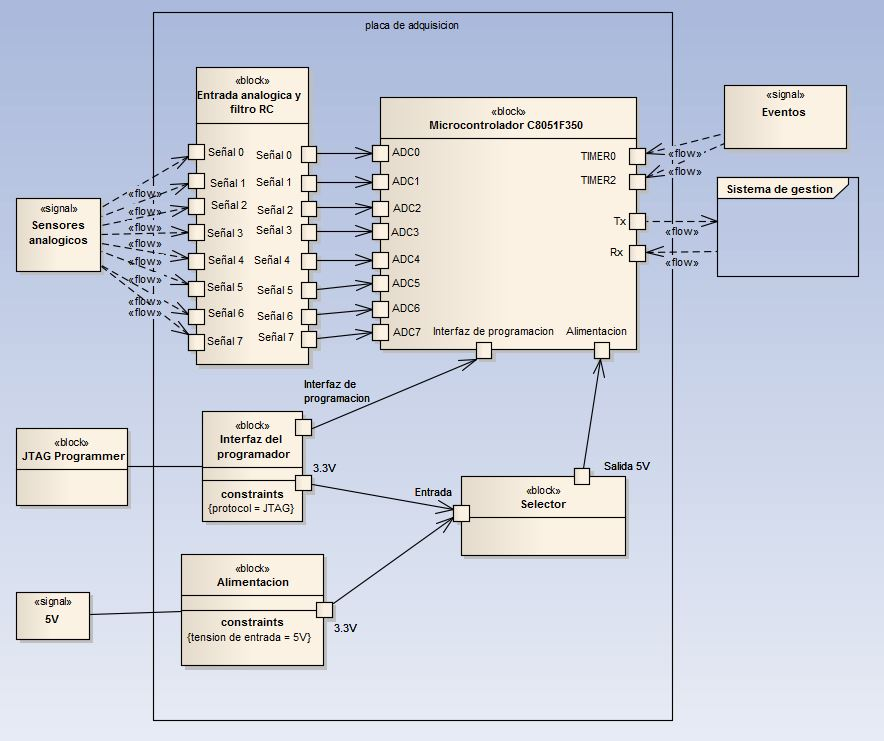
\includegraphics[width=0.50\textwidth, height = 7cm]{BloquesHardw1}
  \caption{Diagrama de Bloque de la Placa.}\label{fig:BloquesHardw1}
\end{figure}

Los bloques en la figura \ref{fig:BloquesHardw1} representan de forma general los distintos módulos a implementar. Las entradas analógicas se introducen al microcontrolador a través de filtros RC (reductores del ruido), para luego pasar al conversor analogico-digital. El bloque GPIO ("Entrada/Salida de proposito general") consiste en un grupo de pines direccionados a distintas entradas del microcontrolador. Estos pines pueden tener funcionalidades generales, y algunos pueden tener otras mas especificas, como ser: contador de eventos, PCA, PWM, etc. En nuestro diseño, separamos aquellos pines especificos que se utilizan como contadores de eventos, y ademas agregamos 4 pines de proposito general, por la eventual necesidad de requerirlos. 

La alimentacion del sistema puede ser suministrada de dos formas posibles: Mediante una fuenta de tension externa de 5V, o por el mismo debugger del microcontrolador. Por la posible necesidad de reprogramar el microcontrolador, decidimos colocar una llave selectora que permite seleccionar la entrada de alimentacion. Por lo que es posible alimentarlo de ambas formas.

%subsection diagra_bloques_hardware (end)

\subsection{Diseño Esquemático}
\label{it3:sub:diseno_esquematico}

El diseño esquematico del circuito fue realizado con la herramienta de software KiCad. Para facilitar la descripcion, seccionamos el circuito final en varios subcircuitos, y los elaboraremos por separado, para luego mostrar el circuito final.

\subsubsection{Entradas Analógicas}
\label{it3:ssub:entradas_analogicas}

Cada una de las 8 entradas analogicas tienen circuitos de conexion similares. La figura \ref{fig:esquematicoFiltro} ilustra el circuito para una de estas entradas. \\

El ruido en el sistema es un factor importante a tener en cuenta. Ingresa por interferencia de señales externas, por temperatura, por la fuente de tension, y por los mismos componentes que conforman el circuito. Como primera medida, cada entrada analogica contiene un filtro RC pasivo que reduce el ruido en una primera instancia. Ademas, el mismo microcontrolador trata el ruido de la señal para mejorar la relacion SNR. \\

En la figura \ref{fig:esquematicoFiltro} se muestra un pin de entrada AI0, que se conecta a la salida de un dispositivo de instrumentacion. La señal de este sensor, se filtra mediante el circuito RC compuesto por una resistencia de 100 Ohms y un capacitor de 0,1 $\mu$F.

\begin{figure}[H]
  \centering
  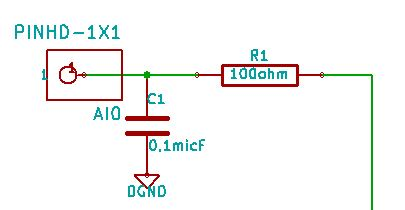
\includegraphics[width=0.70\textwidth, height = 4cm]{esquematicoFiltro}
  \caption{Esquemático del circuito de entrada analógica, más filtro RC pasa-bajo.}\label{fig:esquematicoFiltro}
\end{figure}

%subsubsection entradas_analogicas (end)

\subsubsection{Circuito de interfaz serial}
\label{it3:ssub:circuito_de_interfaz_serial}

La interfaz serial RS-232 es necesaria para el acondicionamiento del canal de datos entre la plataforma y el sistema embebido de destino. En esta seccion elaboramos la construccion del circuito de dicha interfaz. \\

La salida serial del microcontrolador tiene un nivel de tension TTL, insuficiente para un adaptador RS-232, por lo que fue necesario adaptar este nivel para asegurar el correcto envio de datos. El circuito de adaptacion se muestra en la figura \ref{fig:esquematicoMax232}. Contiene un integrado MAX232 que es utilizado ampliamente en la industria para adptar niveles TTL a RS-232. Los pines "XRX1", "XCTS1", "XTX1" y "XRTS1" son los correspondientes al modulo de salida del adaptador serial. \\

Ademas de la adaptacion, colocamos 4 jumpers (JP1, JP2, JP3, JP4) a la entrada del integrado MAX232 en caso en que se requiera la salida TTL del microcontrolador. \\

\begin{figure}[H]
  \centering
  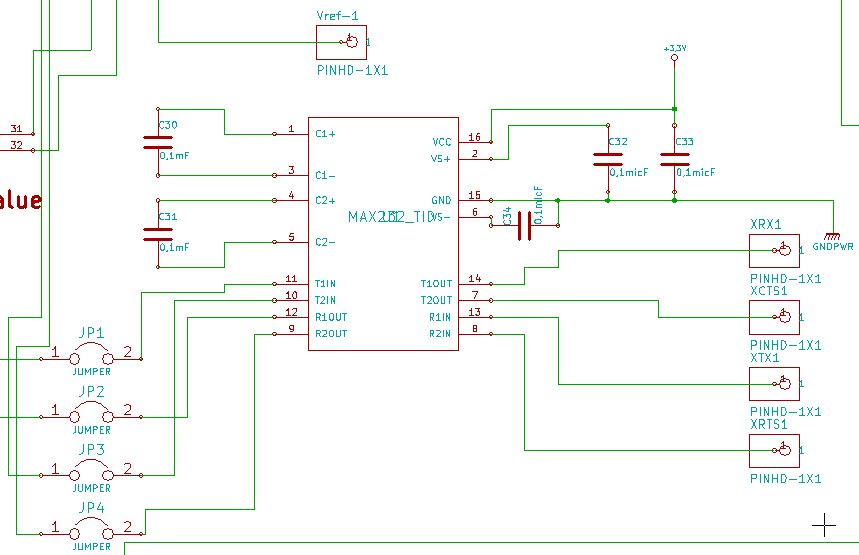
\includegraphics[width=1.0\textwidth, height = 8cm]{esquematicoMax232}
  \caption{Esquemático del Circuito MAX232 .}\label{fig:esquematicoMax232}
\end{figure}

%subsubsection salida_serial (end)

\subsubsection{Circuito de alimentacion}
\label{it3:ssub:circuito_de_alimentacion}

La tension de alimentacion del circuito de la plataforma es de 3,3V. Con el proposito de utilizar una fuente de alimentacion generica de 5V, utilizamos un regulador de tension LM2937 que baja de un nivel de 5V a 3,3V.

Es posible alimentar el circuito mediante una fuente de 5V o el debugger del mismo microcontrolador. Este debugger entrega 3,3V a la salida, por lo que, si el debugger esta conectado como alimentacion, no es necesario utilizar el regulador de tension.

La figura \ref{fig:esquematicoPotencia} muestra el circuito de alimentacion. Colocamos una serie de jumpers que permiten seleccionar si se alimentara el circuito con una fuente de 5V, o el debugger del microcontrolador

\begin{figure}[H]
  \centering
  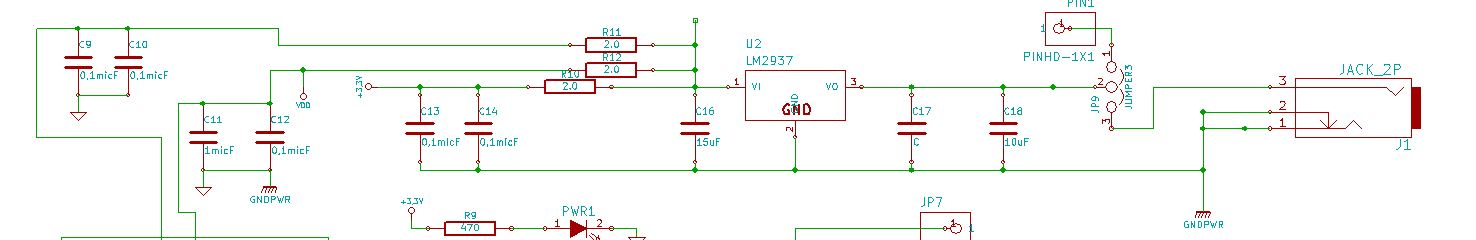
\includegraphics[width=1.0\textwidth, height = 6cm]{esquematicoPotencia}
  \caption{Esquemático del Circuito de Potencia.}\label{fig:esquematicoPotencia}
\end{figure}

%Para poder alimentar al microcontrolador necesitábamos 3.3V así que utilizamos un regulador de tensión (LM2937). El C8051f352 tiene dos entradas de alimentación, una analógica y una digital, ambas con un rango entre 2.9V a 3.6V, ademas la corriente puede variar entre 5.7mA (en estado inactivo) hasta 11.3mA (en estado activo). Es por ello que se colocan las resistencias, y ademas se colocan capacitores en paralelo para disminuir el ruido de entrada.

%subsubsection circuito_potencia (end)

\subsubsection{Diagrama Esquematico Final}
\label{it3:ssub:diagrama_esquematico_final}

De los circuitos descritos anteriormente, se ilustra el circuito final en la figura \ref{fig:EsquematicoCompleto1}

\begin{figure}[H]
\centering
  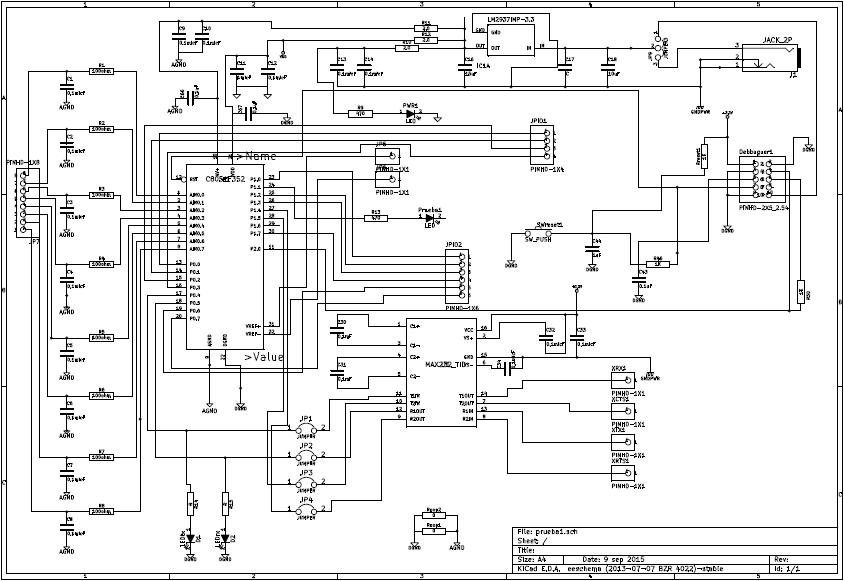
\includegraphics[width=1.10\textwidth, height = 12cm]{EsquematicoCompleto1}
  \caption{Esquemático del Circuito Completo de la placa.}\label{fig:EsquematicoCompleto1}
\end{figure}

%subsubsection esquematico_final_1 (end)

%subsection diseno_esquematico (end)

\subsection{Impresion de circuito en placa de cobre}
\label{it3:sub:impresion_de_circuito_en_placa_de_cobre}

Una plaqueta de circuito impreso (PCB) es una superficie constituida por caminos o pistas de material conductor, laminadas sobre una base no conductora. El circuito que se imprime en un plaqueta se utiliza para interconectar distintos dispositivos electrónicos.

En el Laboratorio de Arquitectura de Computadoras, donde fue realizado este proyecto, esta disponible una maquina fresadora con control numerico por computadora, para la impresión de placas PCB, modelo LPKF E33. El PCB diseñado fue impreso con esta maquina. El software utilizado para la impresion fue ``Circuit Pro'', proveido por los mismos fabricantes de la maquina fresadora. 

La figura \ref{fig:PCB1} ilustra la proyeccion de componentes en el PCB, antes de ser impreso.

\begin{figure}
\centering
  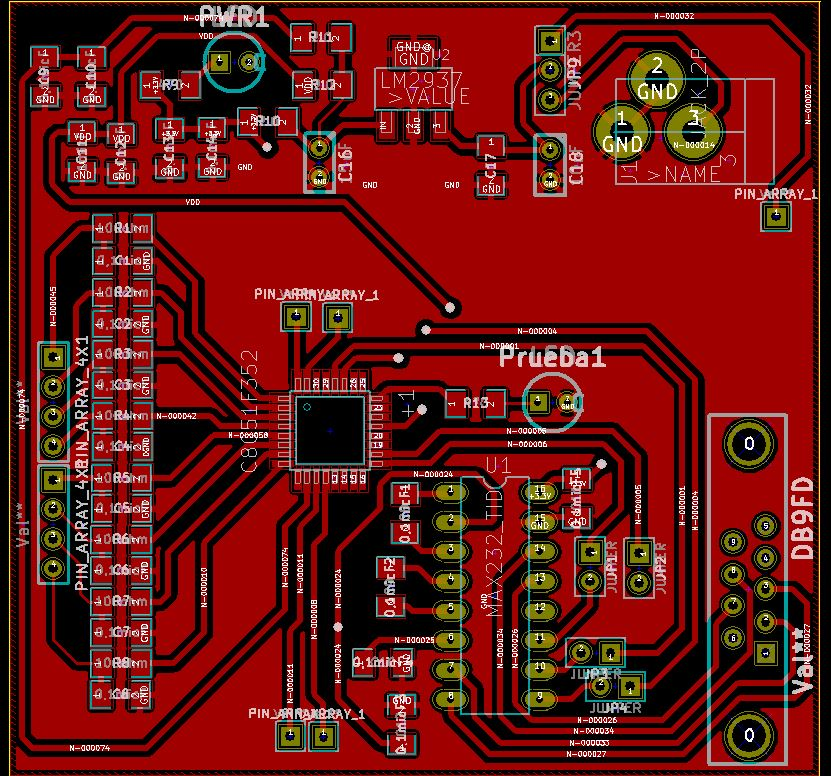
\includegraphics[width=1.10\textwidth, height = 12cm]{PCB1}
  \caption{Esquemático del Circuito Completo de la placa.}\label{fig:PCB1}
\end{figure}


%subsection pcb1 (end)

FALTAN PONER IMAGENES DE LA PLACA IMPRESA CON LOS COMPONENTES SOLDADOS.

% section desarrollo (end)

\clearpage


\section{Pruebas} % (fold)
\label{it3:sec:pruebas}


\begin{table}[h]
\caption{Test de sistema 1}
\label{it3:tab:testsistema1}
\begin{tabular}{p{2cm} p{9cm}}
\multicolumn{2}{c}{\cellcolor[HTML]{68CBD0}{\color[HTML]{000000} Prueba de sistema}} \\                                  
Prueba \#        & 1 \\
\hline
Nombre           & Correcto Diseño de PCB. \\ 
\hline
Requerimientos &   \tabitem Al circuito se le deben poder conectar 8 entradas analógicas. \\
                 & \tabitem Al circuito se le deben poder conectar 4 entradas de eventos digitales externos. \\
                 & \tabitem Las entradas analógicas deben tener filtros para mejorar la inmunidad al ruido. \\
                 & \tabitem Se debe incluir en el diseño el circuito necesario para soportar comunicación vía RS232.                 \\
                 & \tabitem La placa debería poder alimentarse a través de una fuente de tensión externa.  \\                                                                                                                                          
\hline
Descripción      & Se chequea si existen errores en el diseño utilizando el ERC (perfom design rules check) que provee el KiCad. \\
\hline
Pre-condiciones  & \tabitem Componentes colocados y ruteados. \\
                 & \tabitem Pads numerados con sus etiquetas.  \\
\hline
Post-condiciones & El resultado de ERC debe ser cero. \\
\hline
Resultados       & No encontramos errores de diseño en el PCB.                                                                                       
\end{tabular}
\end{table}

\begin{table}[h]
\caption{Test de sistema 2}
\label{it3:tab:testsistema2}
\begin{tabular}{p{2cm} p{9cm}}
\multicolumn{2}{c}{\cellcolor[HTML]{68CBD0}{\color[HTML]{000000} Prueba de sistema}} \\
Prueba \#        & 2 \\
\hline
Nombre           & Correcta impresión de la placa. \\
\hline
Requerimientos &   \tabitem Al circuito se le deben poder conectar 8 entradas analógicas. \\
                 &  \tabitem Al circuito se le deben poder conectar 4 entradas de eventos digitales externos. \\
                 &  \tabitem Las entradas analógicas deben tener filtros para mejorar la inmunidad al ruido. \\
                 &  \tabitem Se debe incluir en el diseño el circuito necesario para soportar comunicación vía RS232.   \\   
                 & \tabitem La placa debería poder alimentarse a través de una fuente de tensión externa.  \\                                                                                                                                                              
\hline
Descripción      & Corroboramos que todas las pistas y que todos los drills se hayan impreso. Luego con un multimetro seteado en continuidad comprobamos que no existan cortocircuitos entre pistas y masa o entre pads y masa. \\
\hline
Pre-condiciones  & \tabitem Placa impresa. \\
                 & \tabitem Multímetro seteado en continuidad.\\
\hline

Post-condiciones & La placa debe tener las mismas pistas que aparecen en el diseño de PCB, y al medir con el tester nunca debe dar continuidad entre masa y pistas, o entre pads y pistas. \\
\hline
Resultados       & Todas las pistas estaban de acuerdo con el PCB. Al medir la continuidad de las pistas se encontraron algunos cortocircuitos producidos por una mala colocación del la plancha al momento de la impresión. Se solucionaron volviendo a imprimir la placa.
\end{tabular}
\end{table}

\begin{table}[h]
\centering
\caption{Test de sistema 3}
\label{it3:tab:testsistema3}
\begin{tabular}{p{2cm} p{9cm}}
\multicolumn{2}{c}{\cellcolor[HTML]{68CBD0}{\color[HTML]{000000} Prueba de sistema}} \\
Prueba \#        & 3 \\
\hline
Nombre           & Correcta soldadura de Componentes \\
\hline
Requerimiento &   \tabitem Al circuito se le deben poder conectar 8 entradas analógicas. \\
                 &  \tabitem Al circuito se le deben poder conectar 4 entradas de eventos digitales externos. \\
                 &  \tabitem Las entradas analógicas deben tener filtros para mejorar la inmunidad al ruido. \\
                &   \tabitem Se debe incluir en el diseño el circuito necesario para soportar comunicación vía RS232.  \\              
                & \tabitem La placa debería poder alimentarse a través de una fuente de tensión externa.  \\

\hline
Descripción      & Se utiliza el multimetro seteado en continuidad para poder chequear si existen cortocircuitos y para saber si todos los componentes estan bien interconectados. \\
\hline
Pre-condiciones  & \tabitem Placa impresa. \\
                 & \tabitem Pistas impresas correctamente. \\
                 & \tabitem Componentes soldados. \\
                 & \tabitem Multimetro seteado en continuidad. \\
\hline 
Post-condiciones &  No deben encontrarse cortocircuitos, y deben comprobarse la continuidad de las interconexiones de componentes. \\ 
\hline
Resultados       & Encontramos cortocircuitos luego de soldar los componentes, al intentar solucionarlo las pistas se rompieron. Para solucionar este problema volvimos a imprimir la placa, realizamos la prueba de sistema 2 de vuelta y soldamos todos los componentes, realizamos esta prueba una vez mas y no encontramos ningún cortocircuito.
\end{tabular}
\end{table}

\begin{table}[h]
\centering
\caption{Test de sistema 4}
\label{it3:tab:testsistema4}
\begin{tabular}{p{2cm} p{9cm}}
\multicolumn{2}{c}{\cellcolor[HTML]{68CBD0}{\color[HTML]{000000} Prueba de sistema}} \\
Prueba \#        & 4 \\
\hline
Nombre           & Correcta Comunicación Con IDE SiliconLabs. \\
\hline
Requerimiento &   \tabitem Se debería poder conectar el debugger del microcontrolador a la placa para poder programarlo. \\
                  &   \tabitem El circuito de programación del microcontrolador debería estar separado la placa principal.  \\                                                                         
\hline
Descripción      & Se utilizo el cable USB con el debugger de SiliconLabs para conectar la placa a la PC. \\
\hline
Pre-condiciones  & \tabitem Placa impresa. \\
                 & \tabitem Pistas impresas correctamente. \\
                 & \tabitem Componentes soldados. \\
                 & \tabitem IDE SiliconLabs instalada en la PC. \\
\hline
Post-condiciones &  Al abrir la IDE y apretar el botón de "Connect" el programa debe reconocer el tipo de microcontrolador al que esta conectado. \\ 
\hline
Resultados       &  Conectamos la placa a la PC y en la IDE apretamos el botón de conectar, con lo que nos reconoció que el micro que se había conectado fue un C8051f352.
\end{tabular}
\end{table}

\begin{table}[h]
\centering
\caption{Test de sistema 5}
\label{it3:tab:testsistema5}
\begin{tabular}{p{2cm} p{9cm}}
\multicolumn{2}{c}{\cellcolor[HTML]{68CBD0}{\color[HTML]{000000} Prueba de sistema}} \\
Prueba \#        & 4 \\
\hline
Nombre           & Correcta programación del microcontrolador. \\
\hline
Requerimiento &   \tabitem Se debería poder conectar el debugger del microcontrolador a la placa para poder programarlo. \\
                  &  \tabitem El circuito de programación del microcontrolador debería estar separado la placa principal. \\
\hline
Descripción      & Se utilizo el cable USB con el debugger de SiliconLabs para conectar la placa a la PC y descargarle un programa .hex al microcontrolador. \\
\hline
Pre-condiciones  & \tabitem Placa impresa. \\
                 & \tabitem Pistas impresas correctamente. \\
                 & \tabitem Componentes soldados. \\
                 & \tabitem IDE SiliconLabs instalada en la PC. \\
                 & \tabitem IDE SiliconLabs reconociendo el C8051f352. \\
\hline

Post-condiciones &  Al abrir la IDE y apretar el botón de "Connect" el programa debe reconocer el tipo de microcontrolador al que esta conectado y luego a traves de la misma IDE o del "Flash Programing Utilitys" cargarle un proframa .hex al c8051f352. \\ 
\hline
Resultados       &  Conectamos la placa a la PC y en la IDE al intentar cargar el programa nos devolvio un error para escribir la flash del microcontrolador.
\end{tabular}
\end{table}




% section pruebas (end)

\section{Resultados} % (fold)
\label{it3:sec:resultados}
La Figura \ref{fig:resultadohardware1} muestra el resultado final de la construccion en PCB de la plataforma.

\begin{figure}[h]
  \centering
  \includegraphics[width=0.80\textwidth, height = 10cm]{resultadohardware1}
  \caption{Placa completa con todo sus componentes soldados.}\label{fig:resultadohardware1}
\end{figure}

En esta iteración cumplimos con los siguientes requerimientos planteados:
\begin{itemize}
  \item Al circuito se le deben poder conectar 8 entradas analógicas.
  \item Al circuito se le deben poder conectar 4 entradas de eventos digitales externos.
  \item Las entradas analógicas deben tener filtros para mejorar la inmunidad al ruido.
  \item Se debe incluir en el diseño el circuito necesario para soportar comunicación vía RS232.
  \item La placa debería poder alimentarse a través de una fuente de tensión externa.
  \item Se debería poder conectar el debugger del microcontrolador a la placa para poder programarlo.
  \item El circuito de programación del microcontrolador debería estar separado la placa principal.
\end{itemize}

En las siguientes imágenes podremos ver el resultado final de la placa.

Pero no pudimos cargarle un programa al c8051f352, como muestra el Test de Sistema 5 \ref{it3:tab:testsistema5} , ya que nos daba error con la escritura en la memoria flash.
% section resultados (end)

% chapter iteracion_3 (end)